\chapter{Experimental Setup}	\label{chapter:experimental_setup}

MABDI was developed and tested in a completely simulated environment for several
reasons. First, all results are repeatable. Having repeatable results is
important for algorithm development because the effects of code changes in the
implementation can be directly correlated to changes in the output. This
facilitates isolation and identification of trouble spots in the code. In
addition, it is possible to test the algorithm in the most ideal environment
before adding complexity. The ability to ramp up the difficulty of the
environment in which MABDI is performing is important for making informed design
decisions. Finally, by performing the analysis in simulation we can quickly see
how the map produced by MABDI compares with the simulated environment. This
comparison is an important tool for development.

In this chapter we will give an overview of the simulation environment, discuss
how noise was generated to mimic the input of a real RGB-D sensor, and look at
the parameters chosen for the experimental runs.

\section{Simulation Overview}

For the experiments, we simulate a sensor moving in a fixed environment along a
defined path. The simulation consists of two main coordinate systems. A
coordinate system fixed to the environment called the global coordinate system
and one attached the origin of the sensor's viewing frustum. Fig.
\ref{fig:simulation_overview} shows the two coordinate systems from two
different vantage points. In the figure red, green, and blue arrows represent
the x, y, and z axis respectively.

\begin{figure}[h]%[thpb]
\centering
  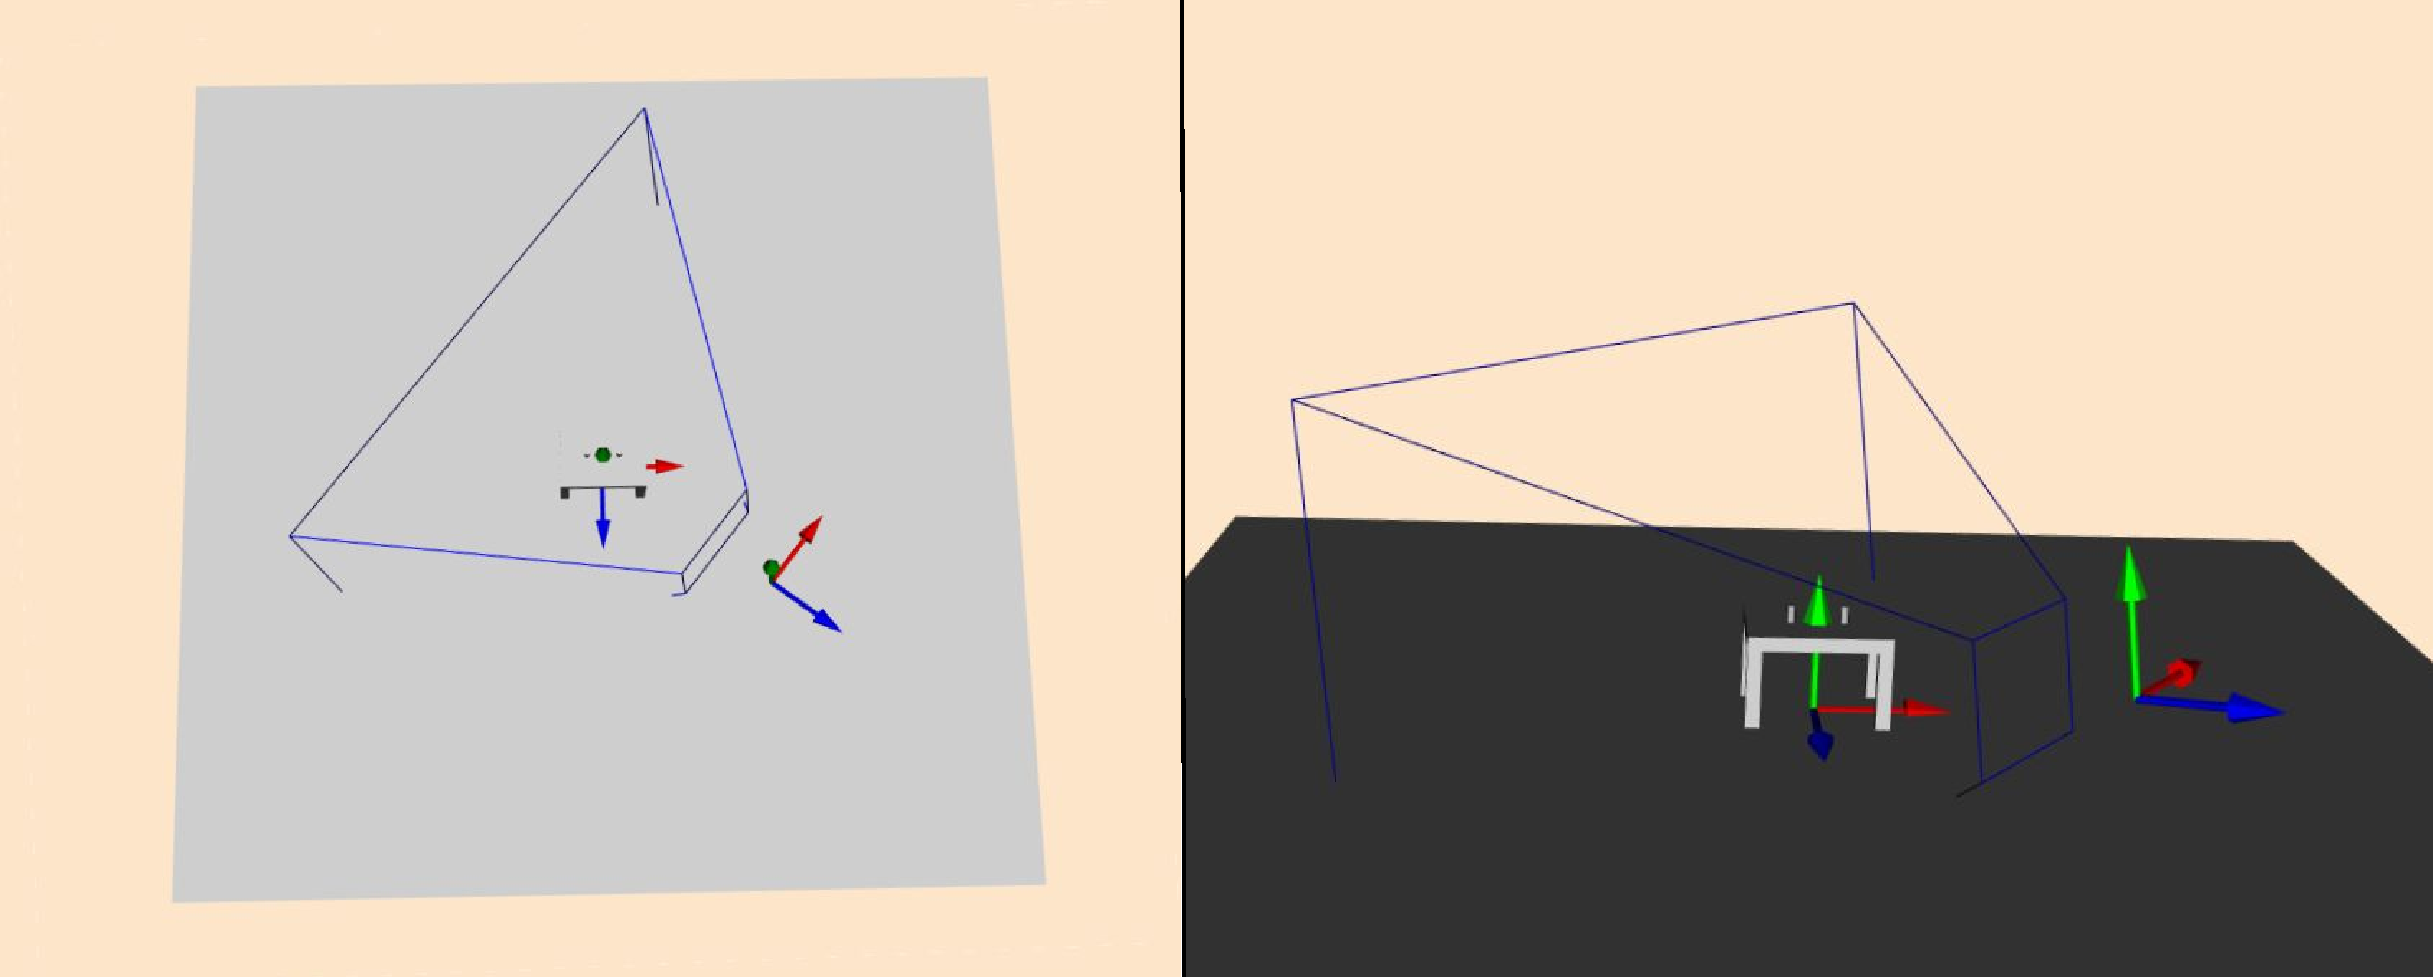
\includegraphics[width=\textwidth]{figures/expsetup_simulation_overview.pdf}
  \caption{Overview of the simulation. Left: Top view. Right: Third person view. }
  \label{fig:simulation_overview}
\end{figure}

\section{Simulating a RGB-D Sensor}

\subsection{Rendering Pipeline}

In order to simulate the depth output of a RGB-D sensor, the environment is
rendered from the sensor's point of view. The rendering process produces a depth
image and this image is used as the simulated output of the sensor. Rendering is
performed by the Open Graphics Library (OpenGL). OpenGL creates a rendering
pipeline that consists of a series of transformations to project 3D global
coordinates to 2D pixel coordinates. A diagram of the rendering pipeline is
shown in Fig. \ref{fig:render_pipeline}. $T_{pcm}$ represents the pinhole
camera model and transforms geometry in the sensor's coordinate system to
homogenous coordinates. The z-component of the homogenous coordinates is what
defines the depth image. Note, the use of a pinhole camera model for simulating
RGB-D output has been validated in the localization work of Fallon
\cite{Fallon2012} and the intrinsic camera parameters of the model were chosen
to replicate the Kinect sensor \cite{sitekinectspecs}.

\begin{figure}[h]%[thpb]
\centering
  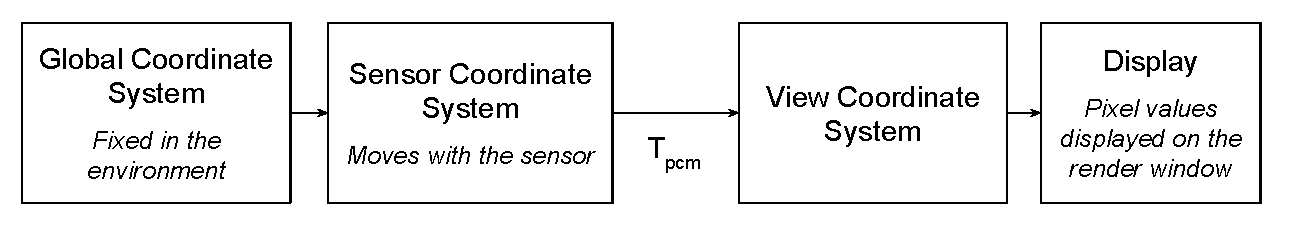
\includegraphics[width=\textwidth]{figures/expsetup_render_pipeline.pdf}
  \caption{Render pipeline: projects 3D global coordinates to 2D pixel coordinates. }
  \label{fig:render_pipeline}
\end{figure}

The pinhole camera transformation, $T_{pcm}$, creates a non-linear relationship
between values in the depth image and their corresponding location in the
sensor's coordinate system. This relationship is visualized in Fig.
\ref{fig:depth_view_to_sensor}.

\begin{figure}[h]%[thpb]
\centering
  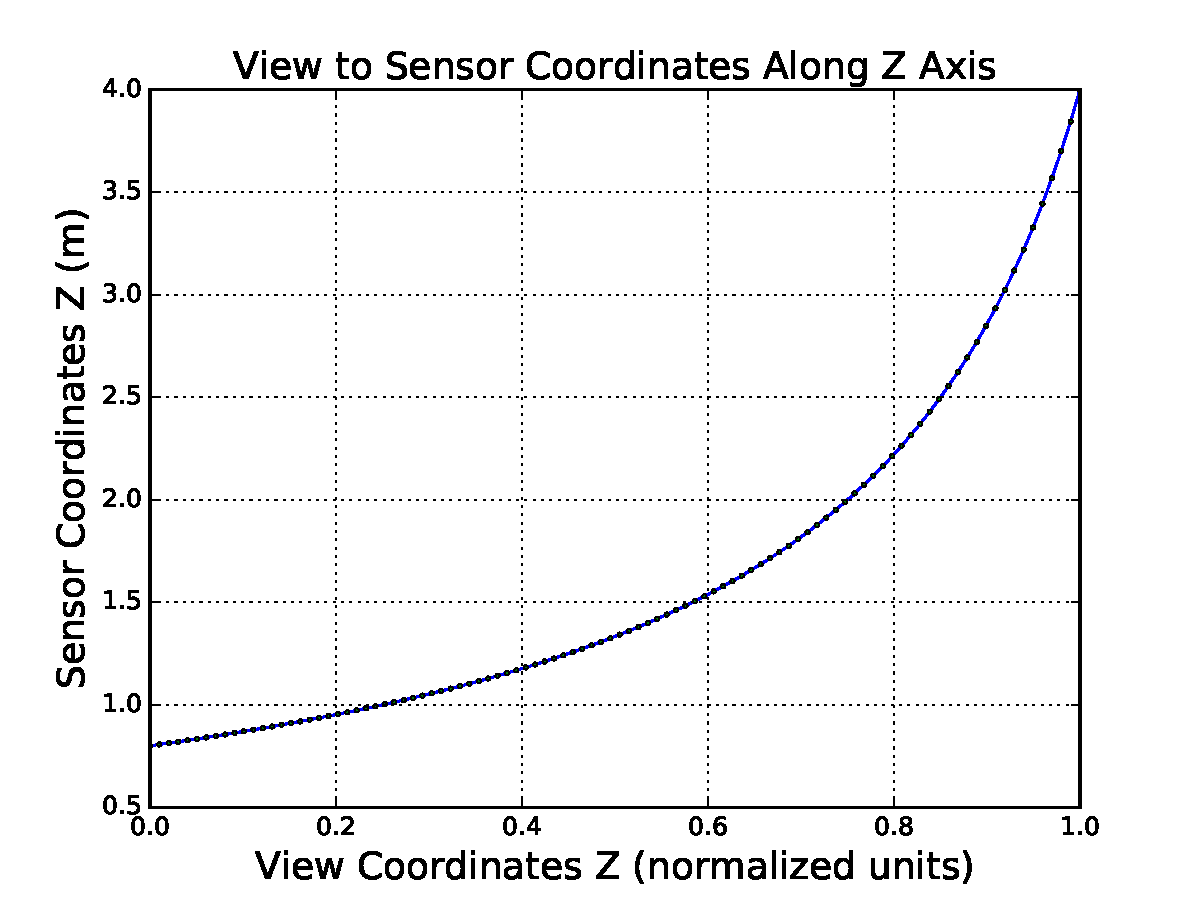
\includegraphics[width=.70\textwidth]
    {figures/expsetup_depth_view_to_sensor.pdf}
  \caption{View coordinates to the sensor's coordinates.}
  \label{fig:depth_view_to_sensor}
\end{figure}

\subsection{Adding Noise to the Depth Image}

% Fully introduce error model, describe that it shows standard deviation as a function of distance
% Define parameters in the error model
To simulate a realistic RGB-D sensor, we add noise to the depth image $D$ with
the goal of approximating RGB-D error models from the literature. Researchers
have created error models to describe the standard deviation of measurement
error found in various RGB-D sensors. For this work, we seek to match the
well-known error model of Khoshelham \cite{Khoshelham2012} that is based on the
original Kinect. The error model is defined in Equation \ref{eqn:k_error_model}.
The equation expresses the standard deviation of error in the z-component of a
point in the sensor's coordinate system $\sigma_z$ (cm) as a function of the
value of the z-component $Z$ (m). Measurements further away from the sensor have
a larger standard deviation of error. The error model is graphed as the red line
in Fig. \ref{fig:depth_noise_error}.

\begin{equation}
  \sigma_z = 1.425\mathrm{e}{-5} \times Z^2
  \label{eqn:k_error_model}
\end{equation}

To approximate a real RGB-D sensor that matches Khoshelham's noise model, noise
is added to the depth image $D$ by sampling a normal distribution and adding the
value to each pixel. as defined in the equation below. The mean of the normal
distribution in Equation \ref{eqn:depth_noise}, $\sigma\mathsmaller{=}0.002$,
was experimentally found to provide a conservative approximation of Khoshelham's
error model.

\begin{equation}
  D_{noisy}(i,j) = D(i,j) + \mathcal{N} (\mu\mathsmaller{=}0, \sigma\mathsmaller{=}0.002)
  \label{eqn:depth_noise}
\end{equation}

In order to compare the magnitude of the standard of deviation of error used in
our experiments with that of Khoshelham's error model, we graph them on the same
plot (Fig. \ref{fig:depth_noise_error}). Each line shows how the measurement's
standard deviation of error changes as the point moves along the z axis in the
sensor's coordinate system. The standard deviation of error simulated in our
experiments is larger than that defined by Khoshelham's model for points within
the sensor's range. Therefore, our experiments are a conservative estimate of
the error found in real world RBG-D sensors.

\begin{figure}[h]%[thpb]
\centering
  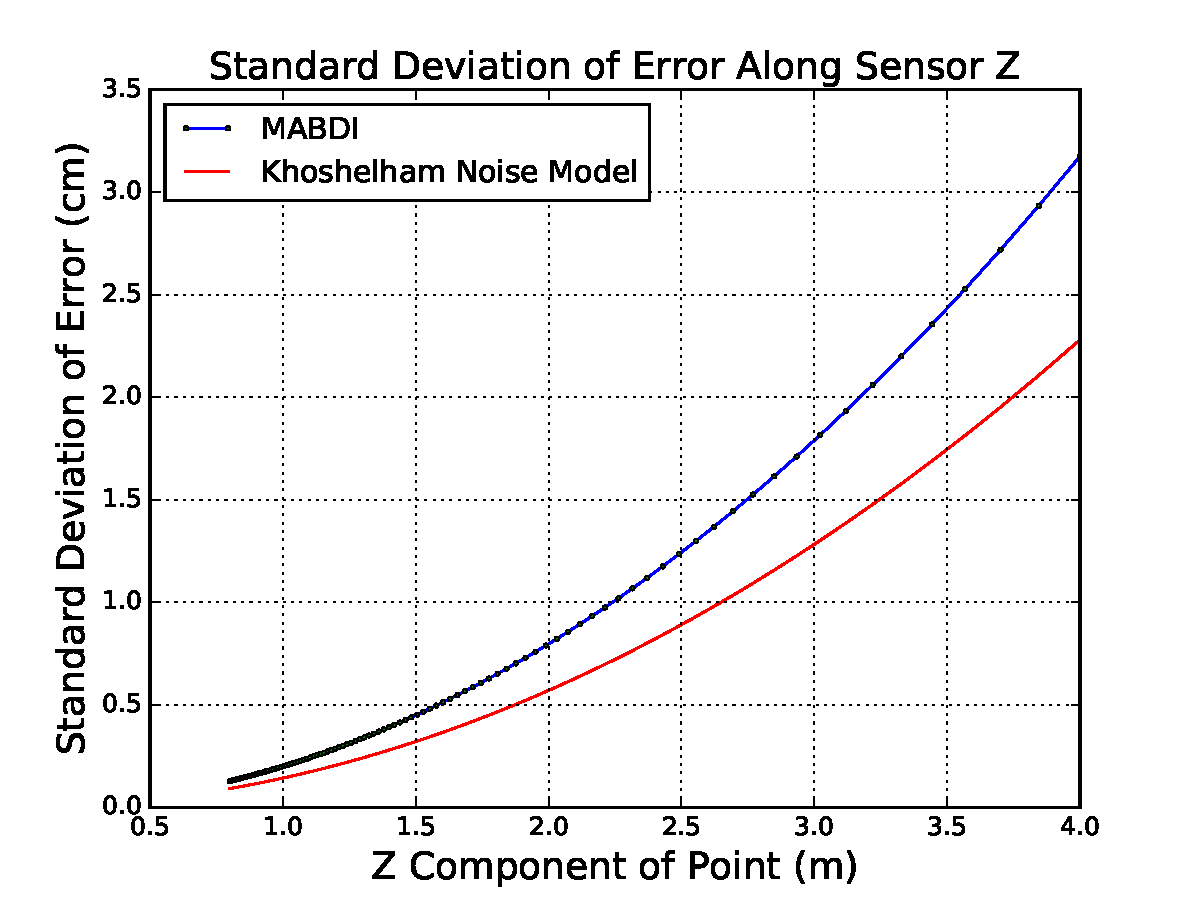
\includegraphics[width=.70\textwidth]{figures/expsetup_noise_error.pdf}
  \caption{Comparison of standard deviation of the error used in the MABDI simulation and the error model from Khoshelham.}
  \label{fig:depth_noise_error}
\end{figure}

\section{Sensor Path}

All experimental runs define a helical path for the sensor to follow during the
simulation. The path is shown in Figure \ref{fig:sensor_path}. The blue line
indicates the path and the pink points indicate where the sensor stops along the
path. The path circles the objects in the environment twice. A helical path was
chosen because it returns to a part of the environment that has already been
mapped and is thus ``known'' to the algorithm. Also, because the path is a
helix and not just a circle, the sensor views the environment from a slightly
different position on each pass.

\begin{figure}[h]%[thpb]
\centering
  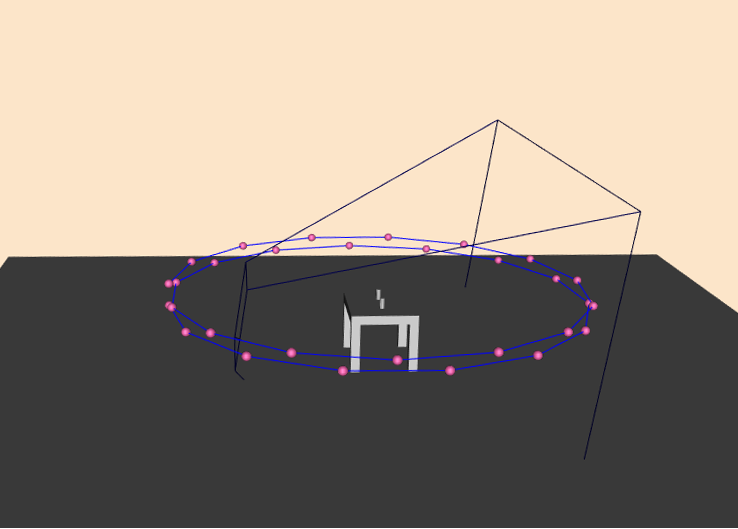
\includegraphics[width=.70\textwidth]{figures/expsetup_path.png}
  \caption{View of the sensor path. The blue line indicates the sensor path and the pink points indicate where the sensor stops along the path.}
  \label{fig:sensor_path}
\end{figure}

\section{Simulation Parameters}

The simulation was designed to be highly configurable and is implemented by a
class named MabdiSimulate. This class is responsible for connecting all the
components expressed in Fig. \ref{fig:software} of Chapter
\ref{chapter:approach}. MabdiSimulate is initialized with parameters that
control all aspects of the simulation. Parameters of a particular importance are
discussed in more detail here:

\begin{itemize}
    \item Environment - This parameter specifies the environment used to generate
    the simulated depth images. \textit{Table} is an environment consisting of a
    table and two cups placed on the table. The table is 1 meter tall.
    \textit{Bunnies} is an environment consisting of three bunnies that are
    around 1.5 meters tall. These bunnies are created using the Stanford Bunny
    \cite{Turk1994}, a well known data set in computer graphics.
    \item Noise - If true, adds noise to the depth image of the simulated sensor.
    \item Dynamic - If true, adds an object during the simulation. In the case
    of this analysis, a third bunny is added half-way through the simulation.
    \item Iterations - The number of times MABDI will run. This number is equal to the number of stops the sensor makes along the path because every time the sensor stops MABDI is run to update the global mesh. Figure \ref{fig:sensor_path} shows sensor stops along the sensor path.
\end{itemize}

We will be exploring three experimental runs to demonstrate the
ability of the MABDI implementation to generate valid results. Additionally, the
experimental runs will be able to show the capabilities of the MABDI algorithm
such as handling object addition in the environment.

\begin{table}[h]
  \caption{Description of the experimental runs.}
  \label{tab:run}
  \begin{footnotesize}
  \begin{center}
    \begin{tabular}{|l|c|c|c|c|}
    \hline
           & Environment & Noise   & Dynamic & Iterations \\\hline
    Run 1	 & Table       & False   & False   & 30 \\
    Run 2  & Bunnies     & True    & False   & 50 \\
    Run 3  & Bunnies     & True    & True    & 50 \\
    \hline
    \end{tabular}
  \end{center}
  \end{footnotesize}
\end{table}
